\chapter{Моделирование деградации РТГС на основе $Al_{x}Ga_{1−x}As$}
На основе выше исследованных параметров и полученных моделей получим модель деградации РГТС на основе $AlGaAs$.

В схема исследуемой на диффузионное размытие модели приведена на рис.\ref{fig:RTHSModelDiff}

\begin{figure}
	\centering
	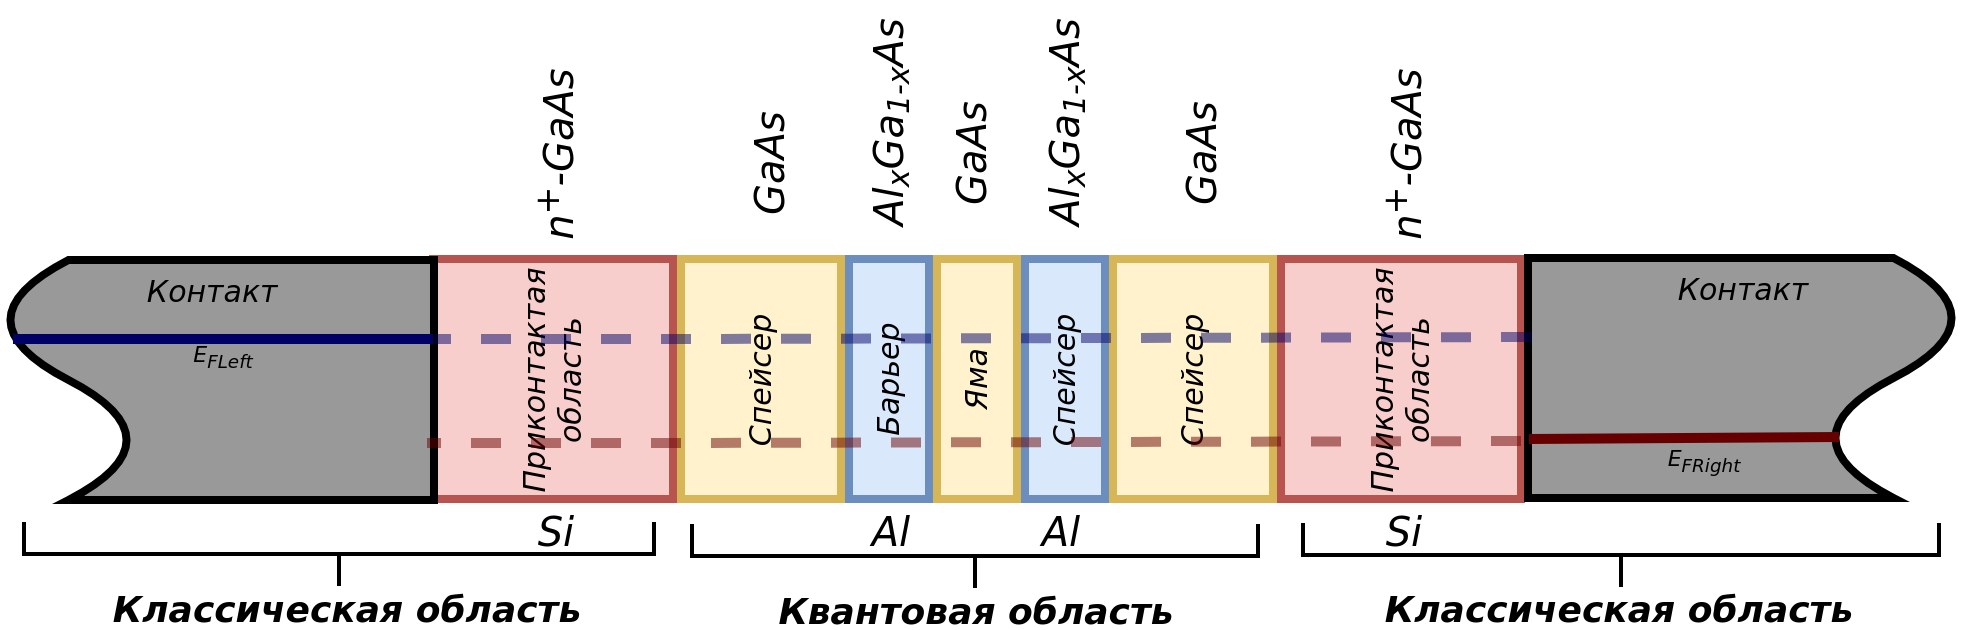
\includegraphics[width=0.9\linewidth]{assets/RTHSModelDiff}
	\caption{Структура РТГС для моделирования диффузии}
	\label{fig:RTHSModelDiff}
\end{figure}

В данной модели возможны:
\begin{itemize}
	\item Диффузия $Al$ из барьеров в яму;
	\item Диффузия $Si$ из приконтактных областей в активную область.
\end{itemize}

Факторы влияющие на деградацию GaAs гетероструктуры:
\begin{itemize}
	\item Технологические: \begin{itemize}
		\item МЛЭ (Для РТД $t\approx560$ секунд, $T\approx550$--$650^{\circ}$C);
		\item Отжиг (Для РТД $t\approx30$ секунд, $T\approx800^{\circ}$C);
		\item Отжиг металлических контактов (Для РТД $t\approx15$--$120$ секунд, $T\approx350$--$470^{\circ}$C).
	\end{itemize}
	\item Эксплуатационные:
	\begin{itemize}
		\item Температурная и временная нагрузка ($t\approx 10$ лет, $T\approx25$--$100^{\circ}$C).
	\end{itemize}
\end{itemize}

Рассмотрим диффузионное размытие активной области и проникновение легирующий примеси отдельно.

Размеры модели:
\begin{itemize}
	\item Спейсер: $a = 10$ монослоев;
	\item Барьер: $b = 6$ монослоев;
	\item Яма: $c = 6$ монослоев;
	\item Приконтактная область: $r = 20$ монослоев.
\end{itemize}

\begin{figure}
	\centering
	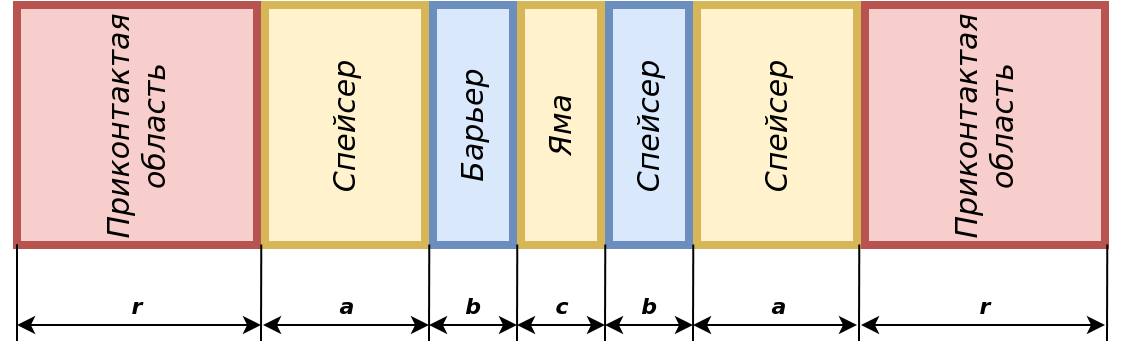
\includegraphics[width=0.99\linewidth]{assets/RTHS}
	\caption{Размеры РТГС}
	\label{fig:RTHS}
\end{figure}

\section{Диффузия в активной области}
Диффузионное размытие активной области в случаи чистых полупроводников подчиняется (\ref{eq:DConst}). Коэффициент диффузии постоянен и скорость ухода части $Al$ с границ активной области равен скорости их прихода -- это соответствует конечно-разностной схеме (\ref{eq:DDiffConst}).

Первый этап деградации --- это подогрев (в худшем случае) до $650^{\circ}$C РТГС для МЛЭ. Скорость процесса $1$монослой/c. Будет нагревать подложку на протяжении:

\begin{itemize}
	\item $0$ секунд;
	\item $560$ секунд;
	\item $1200$ секунд;
	\item $7200$ секунд.
\end{itemize}

Результат деградации от МЛЭ на рис.\ref{fig:DA650} получены с помощью лист.\ref{lst:Da} и лист.\ref{lst:DaDiff}

\begin{figure}[h!]
	\centering
	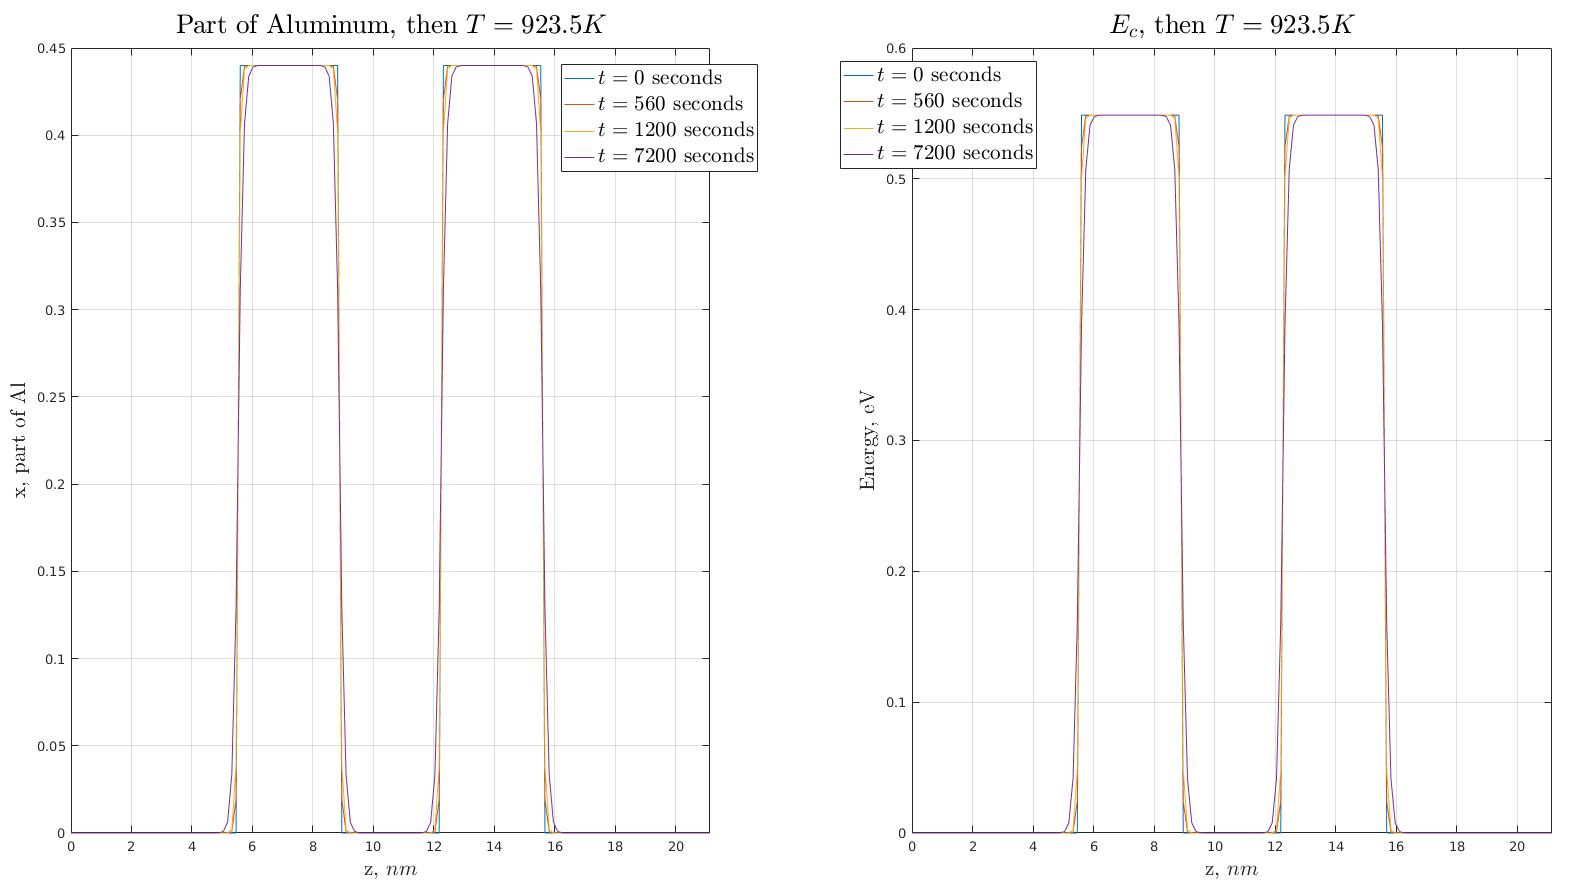
\includegraphics[width=0.99\linewidth]{DA650}
	\caption{Расплытие активной области при МЛЭ}
	\label{fig:DA650}
\end{figure}

Второй этап деградации -- это высокотемпературный отжиг при $T=800^{\circ}$C. Будем нагревать подложку в течении:

\begin{itemize}
	\item $0$ секунд;
	\item $15$ секунд;
	\item $30$ секунд;
	\item $50$ секунд.
\end{itemize}

Результат деградации от отжига на рис.\ref{fig:DA800} получены с помощью лист.\ref{lst:Da} и лист.\ref{lst:DaDiff}

\begin{figure}[h!]
	\centering
	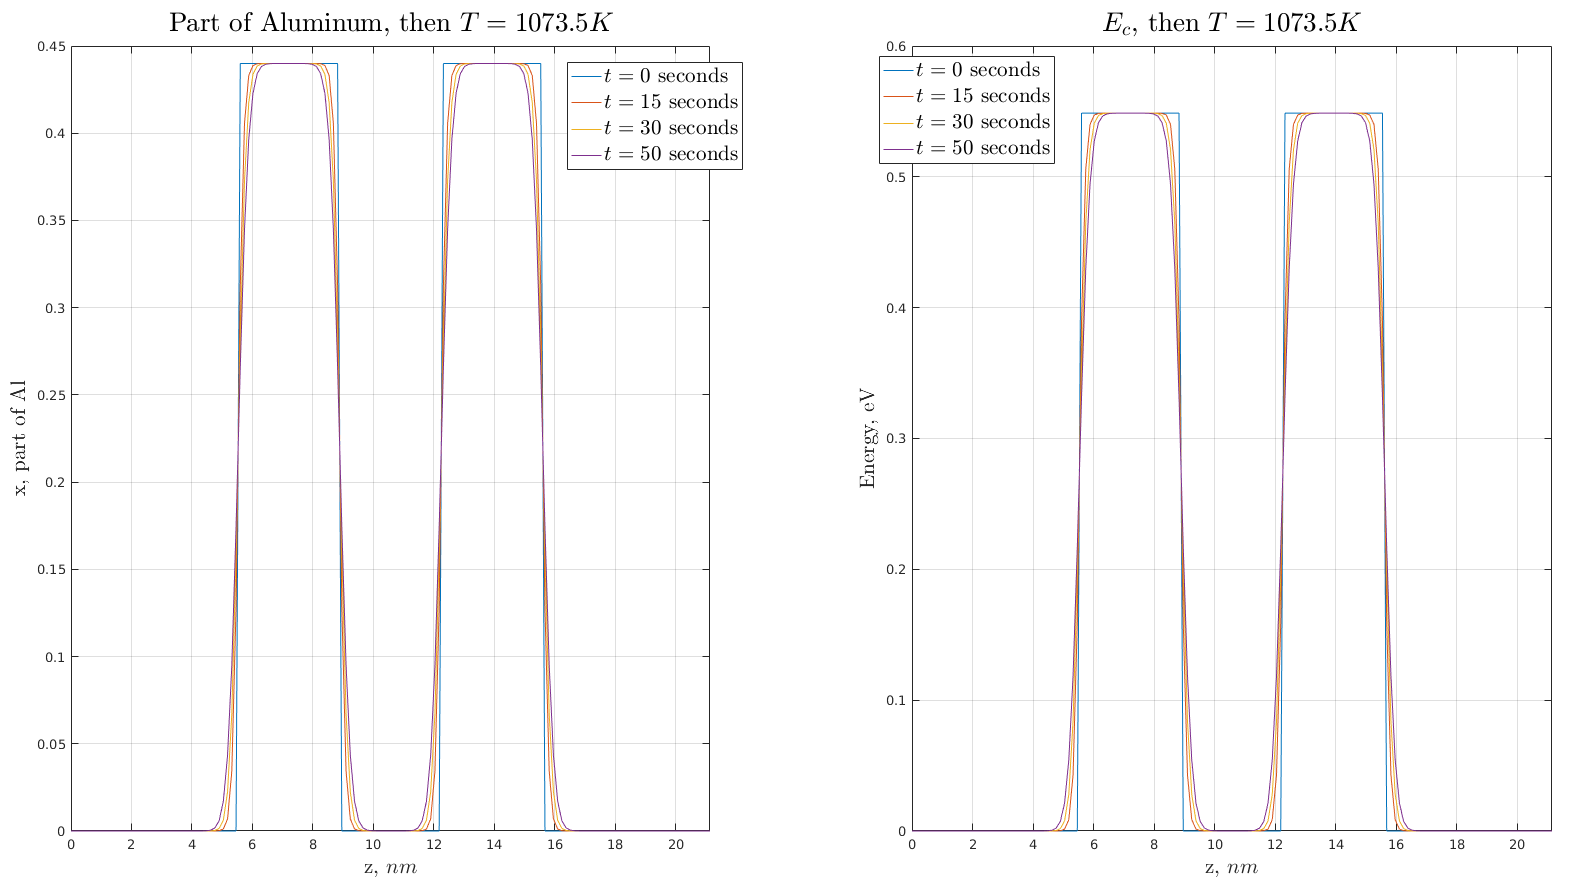
\includegraphics[width=0.99\linewidth]{DA800}
	\caption{Расплытие активной области при отжиге}
	\label{fig:DA800}
\end{figure}

Исходя из результатов моделирования деградации активной области при МЛЭ --- результатами деградации при отжиге металлических контактов можно пренебречь.

В ходе термической деградации при МЛЭ (рис.\ref{fig:DA650}) и отжиге ГС (рис.\ref{fig:DA800}) профиль концентрации $Al$ сглаживается.

Результаты моделирования деградации ГС представлены на рис.\ref{fig:DA100} при $T=100^{\circ}$C, получены с помощью лист.\ref{lst:Da} и лист.\ref{lst:DaDiff}. Времени эксплуатации:

\begin{itemize}
	\item $0$ лет;
	\item $1$ год;
	\item $5$ лет;
	\item $15$ лет.
\end{itemize}

\begin{figure}[h!]
	\centering
	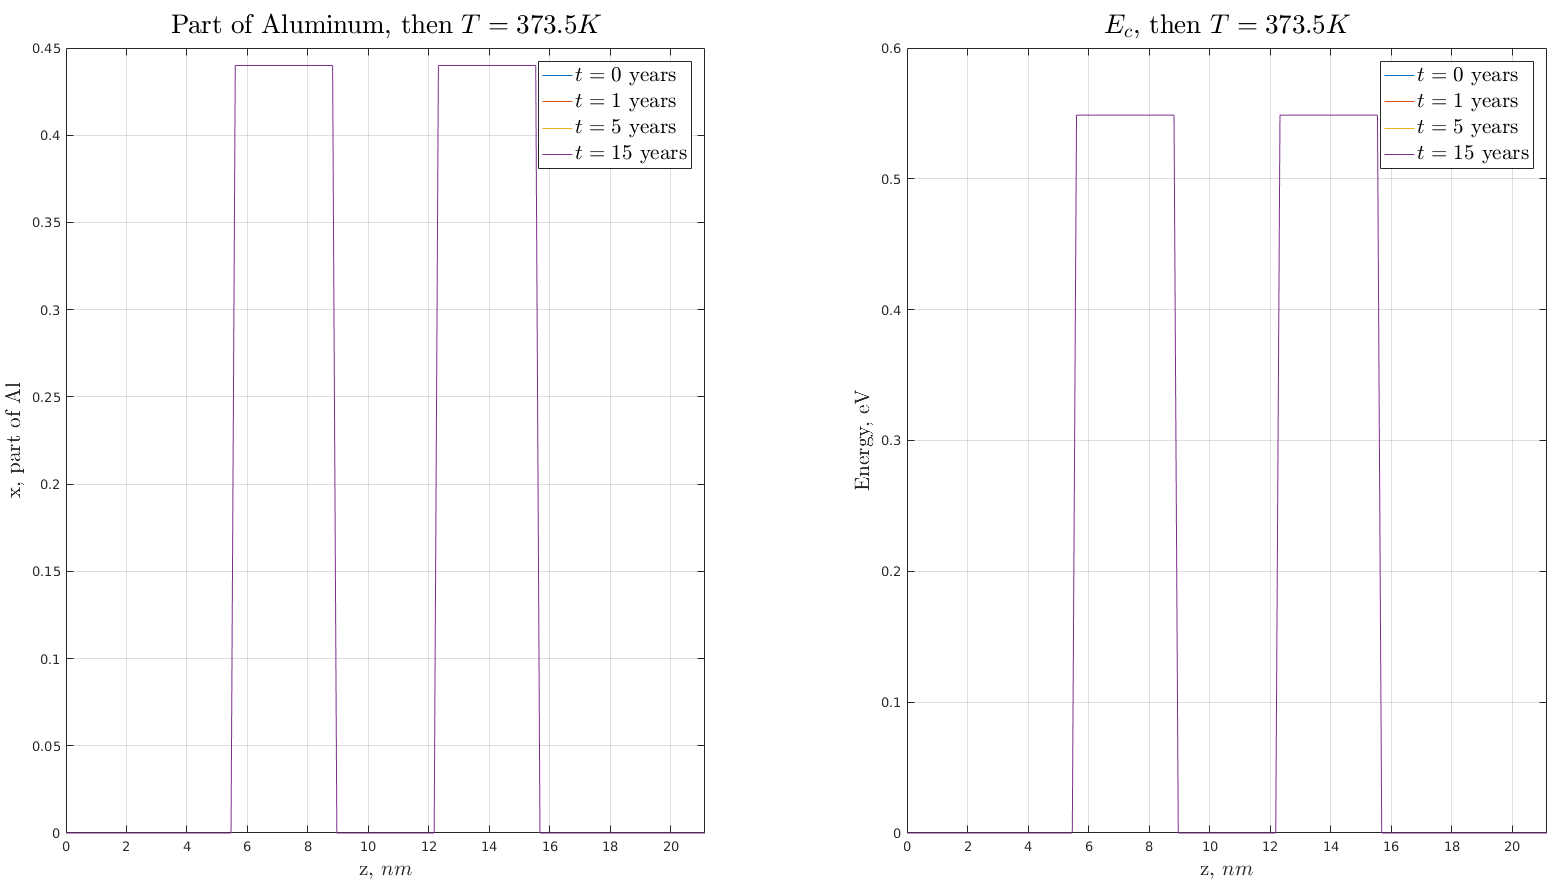
\includegraphics[width=0.7\linewidth]{DA100}
	\caption{Расплытие активной области при отжиге}
	\label{fig:DA100}
\end{figure}

Активная область при такой такой температуре не деградирует.

Так как невозможно получить чистый полупроводник, в нем всегда присутствует донорная примесь, которая увеличивает скорость диффузии, что соответствует (\ref{eq:DNd}).

Рассмотрим деградацию при МЛЭ с теми же условиями, но при $Nd = 5*ni$ (см рис.\ref{fig:DANd650}) получены с помощью лист.\ref{lst:DaNd} и лист.\ref{lst:DaNdDiff}.

\begin{figure}[h!]
	\centering
	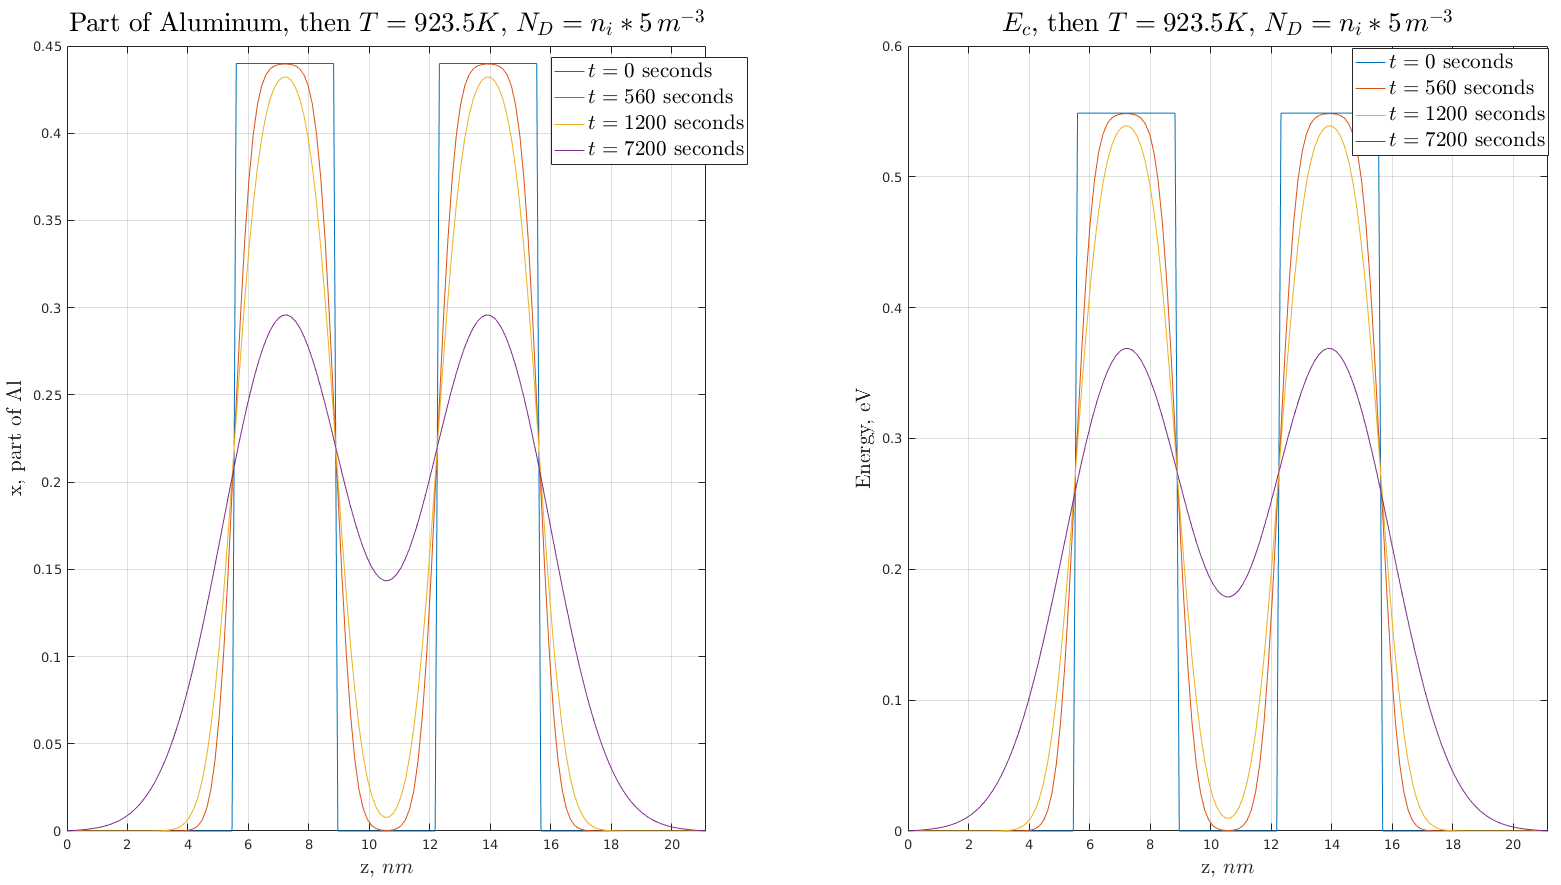
\includegraphics[width=0.99\linewidth]{DANd650}
	\caption{Расплытие активной области при МЛЭ и $Nd = 5*ni$}
	\label{fig:DANd650}
\end{figure}

Рассмотрим деградацию при отжиге с теми же условиями, но при $Nd = 1.5*ni$ (см рис.\ref{fig:DANd800}) получены с помощью лист.\ref{lst:DaNd} и лист.\ref{lst:DaNdDiff}.

\begin{figure}[h!]
	\centering
	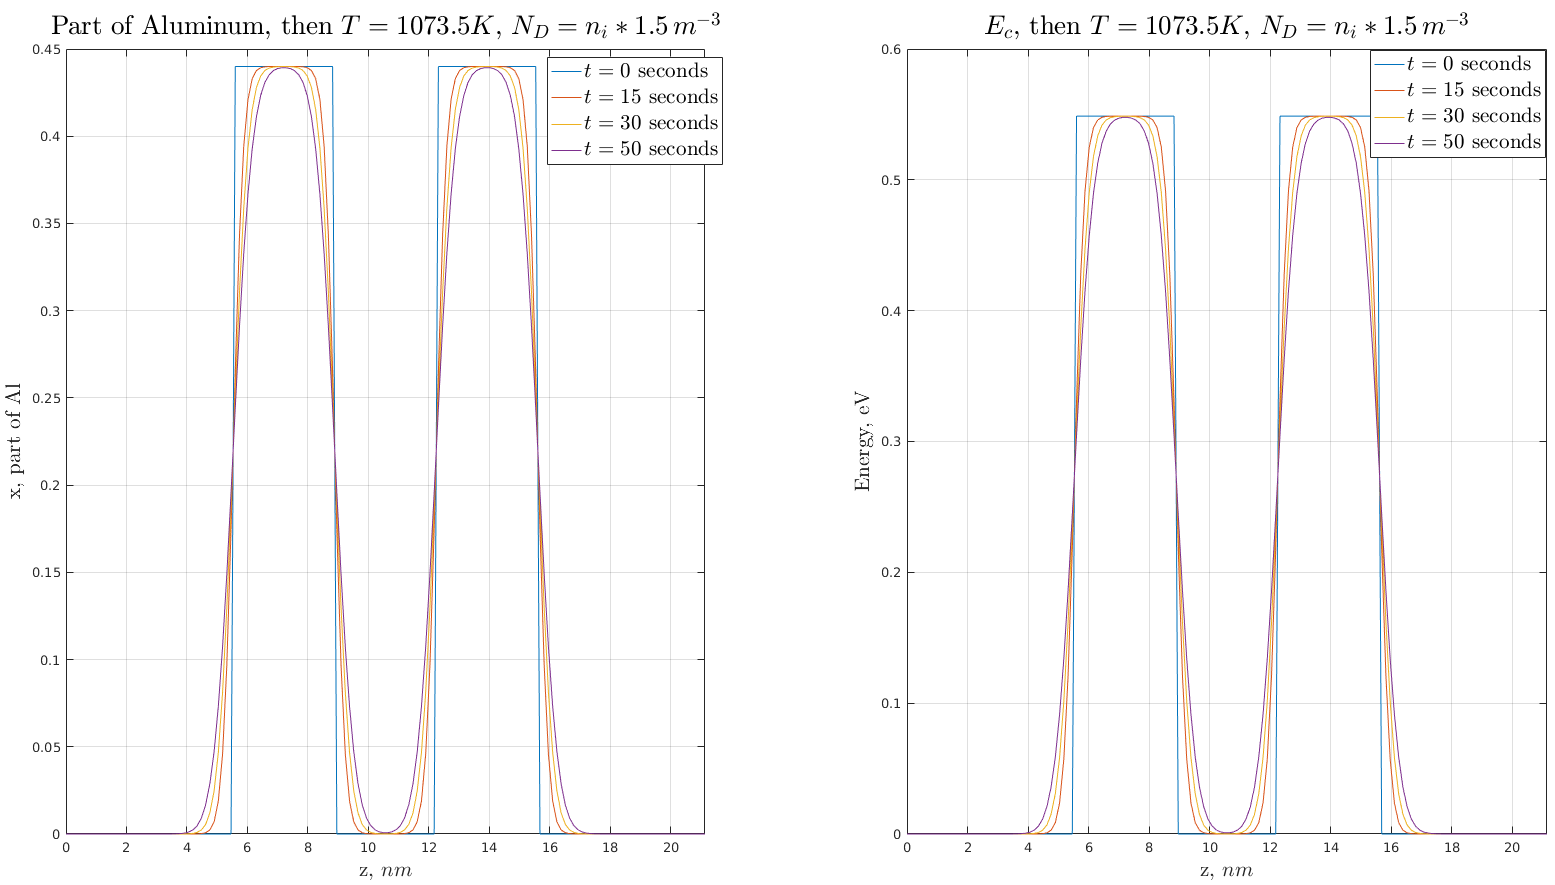
\includegraphics[width=0.99\linewidth]{DANd800}
	\caption{Расплытие активной области при МЛЭ и $Nd = 1.5*ni$}
	\label{fig:DANd800}
\end{figure}


\subsection{Вывод}
Термическая деградация активной области существенна при отжиге и МЛЭ, при этом профиль концентрации $Al$ сглаживается и нельзя выделить явно преобладающего фактора.

При наличии загрязнения (донорной примеси) в материале из которого изготавливается РГТС (РТД) профиль концентрации деградирует существенно, при этом преобладают уменьшение глубины ямы и уширение потенциального барьера.